\section{File Format and Decompression for PFSS Fieldline Data}
This section describes the file format and decompression algorithm for the fieldline data. The data is saved in the FITS file format \cite{website:fits} and compressed with RAR \cite{website:rar}. 

To decompress the data do these steps
\begin{enumerate}
	\item decompress the data with RAR.
	\item Read the FITS file. The content of the FITS file is described in subsection \ref{anhang:format:content}.
	\item Decode Bytes with the algorithm specified in section \ref{anhang:format:encodings}.
	\item Split up the data into the corresponding fieldlines. This step is described in-depth in subsection \ref{anhang:format:content:split}.
	\item Decode predictive coding described in section \ref{anhang:format:prediction}.
\end{enumerate}

\subsection{FITS Content}\label{anhang:format:content}
The FITS file is composed of the header and the body. The content of the header and body are described in table \ref{anhang:format:header} and \ref{anhang:format:body}. \emph{NOTE: The content of the (table \ref{anhang:format:body}) is encoded. The raw Bytes have to be retrieved and decoded before use.} The Byte decoding is described in subsection \ref{anhang:format:encodings}.

\begin{table}[!htbp]
\center
\begin{tabular}{|c|c|c|}
	\hline
	Name  & Datatype & Content Description	\\\hline
    b0 & Float  & Latitude to Earth\\
    l0 & Float & Longitude to Earth\\
    Q1 & Float & Quantization Coefficient 1\\
    Q2 & Float & Quantization Coefficient 2\\
    Q3 & Float & Quantization Coefficient 3\\\hline
\end{tabular}
\caption{Header of the FITS File}
\label{anhang:format:header}
\end{table}

\begin{table}[!htbp]
\center
\begin{tabular}{|c|c|c|}
	\hline
	Name  & Encoding & Content Description	\\\hline
    LENGTH & Adaptive Unsigned & Length of each fieldline\\
    X & Adaptive Signed & X channel of all fieldlines\\
    Y & Adaptive Signed & Y channel of all fieldlines\\
    Z & Adaptive Signed & Z channel of all fieldlines\\\hline
\end{tabular}
\caption{Body of the FITS File}
\label{anhang:format:body}
\end{table}

\subsubsection{Splitting up the body} \label{anhang:format:content:split}
After decoding the body the channels X, Y and Z data have to be split up to their corresponding fieldlines. The decoded LENGTH describes the number of data points which belong to the first fieldline. An example is is illustrated in table \ref{anhang:format:content:split:illustration}.

\begin{table}[!htbp]
	\center
	\begin{tabular}{|c||c|c|c|c}
	\hline
		decoded LENGTH & 4 & 3 & 18 & \ldots\\\hline
	\end{tabular}
	\\
	[\baselineskip]
	\begin{tabular}{|c||c|c|c|c||c|c|c||c}
	\hline
		 & \multicolumn{4}{|c||}{first fieldline} & \multicolumn{3}{|c||}{second fieldline} & \multicolumn{1}{|c}{\ldots}\\\hline
		decoded X & $x_0$ & $x_1$ & $x_2$ & $x_3$ & $x_4$ & $x_5$ & $x_6$ & \ldots \\
		decoded Y & $y_0$ & $y_1$ & $y_2$ & $y_3$ & $y_4$ & $y_5$ & $y_6$ & \ldots \\
		decoded Z & $z_0$ & $z_1$ & $z_2$ & $z_3$ & $z_4$ & $z_5$ & $z_6$ & \ldots \\\hline
	\end{tabular}
	\caption{Illustration of how the body has to be split up}
	\label{anhang:format:content:split:illustration}
\end{table}

\pagebreak
\subsection{Byte Encoding} \label{anhang:format:encodings}
The Byte encoding which is in use for adapts to the number of Bits needed to represent a value. Hence the name ''Adaptive Precision Encoding''. Two implementations are in use: the signed and unsigned variant. The ''Unsigned Adaptive Precision Encoding'' is illustrated in table \ref{anhang:format:encodings:adaptiveUnsigned} and the signed version in table \ref{anhang:format:encodings:adaptive}.

The first Bit of the ''Unsigned Adaptive Precision Encoding'' is the ''Continue Flag''. If the "Continue Flag" is set, then the next Byte also belongs to the value. If the ''Continue Flag'' is not set then the next Byte belongs to a new value. The Bytes are written in Big-Endian\cite{wiki:endianess} convention. Which means that the first data Bit is the Most-Significant-Bit.

The ''Signed Adaptive Precision Encoding'' only has one difference when compared to the unsigned encoding: The first Byte of a value carries the ''Sign Flag'' as shown in table \ref{anhang:format:encodings:adaptive}. If the following Byte belongs to the same value then the encoding of the second Byte is identical to the unsigned encoding (see table \ref{anhang:format:encodings:adaptiveUnsigned}).

\textbf{Unsigned Adaptive Precision Encoding}\\
\begin{table}[!htbp]
	\center
	\begin{tabular}{|c|c|c|c||c|c|c|c|}
	\hline
	\multicolumn{8}{|c|}{Byte}\\\hline
	Continue Flag & X & X & X & X & X & X & X \\\hline
	\end{tabular}
	\caption{Unsigned Adaptive Byte Encoding. X are data Bits.}
	\label{anhang:format:encodings:adaptiveUnsigned}
\end{table}

\textbf{Signed Adaptive Precision Encoding}\\
\begin{table}[!htbp]
	\center
	\begin{tabular}{|c|c|c|c||c|c|c|c|}
	\hline
	\multicolumn{8}{|c|}{Byte}\\\hline
	Continue Flag & Sign Flag & X & X & X & X & X & X \\\hline
	\end{tabular}
	\caption{Signed Adaptive Byte Encoding of the First Byte.  X are data Bits.}
	\label{anhang:format:encodings:adaptive}
\end{table}

Here is an example implementation of the ''Signed Adaptive Precision Encoding'':\\
\lstinputlisting[language=Java]{./source/byteDecoding.txt}

\pagebreak
\subsection{Decode Prediction}\label{anhang:format:prediction}
Here a recursive algorithm is used to predict the content of a channel. The prediction assumes that the mid-value of the channel is on a straight line between the start and end value. Only the error of the prediciton is saved. The figure \ref{anhang:prediction:step1} illustrates this. After the first prediction the algorithm is repeated recursively for the two new segment. The figure illustrates \ref{anhang:prediction:step2} the second recursive step. The recursion stops when all values in a channel have been predicted.

\begin{figure}[!htbp]
	\center
	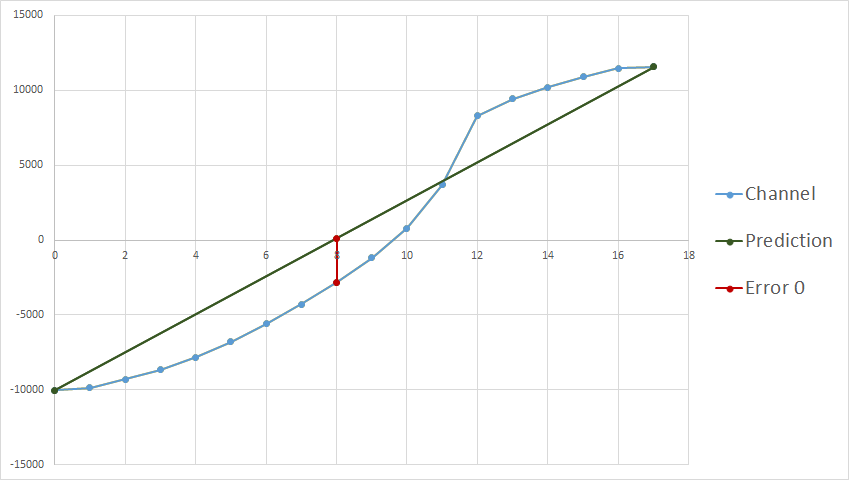
\includegraphics[width=1\textwidth,keepaspectratio]{./pictures/anhang/prediction0.png}
	\caption{First recursive step.}
	\label{anhang:prediction:step1}
\end{figure}
\begin{figure}[!htbp]
	\center
	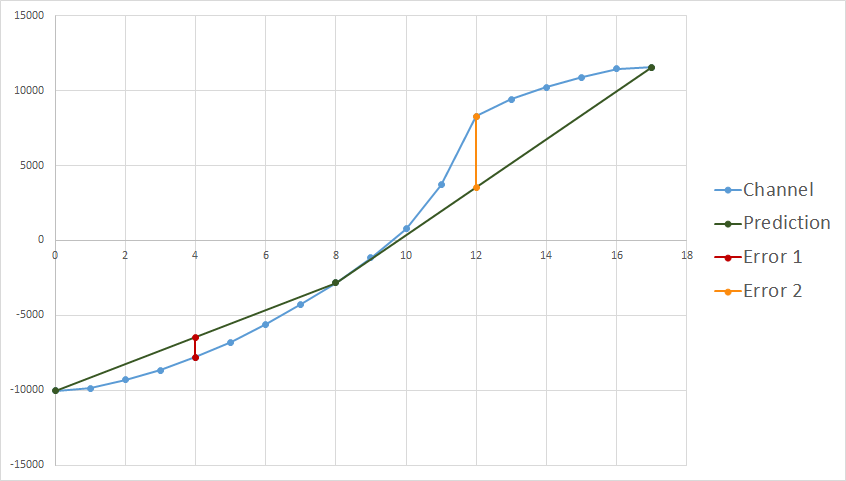
\includegraphics[width=1\textwidth,keepaspectratio]{./pictures/anhang/prediction1.png}
	\caption{Second recursive step.}
	\label{anhang:prediction:step2}
\end{figure}

After Byte decoding and splitting, a channel contains the start and end value and the prediction error as illustrated in table \ref{anhang:format:prediction:content}.
\begin{table}[!htbp]
	\center
	\begin{tabular}{|c|c|c|c|c|c|}
		\hline
		\multicolumn{6}{|c|}{Channel}\\\hline
		start value & endvalue & Error 0 & Error 1 & Error 2 & \ldots \\\hline
	\end{tabular}
	\caption{Content of a channel}
	\label{anhang:format:prediction:content}
\end{table}

The content of the channel is quantized. The content has to be multiplied with the quantization factors $Q_1$,$Q_2$ and $Q_3$ from the FITS file header (see table \ref{anhang:format:header}):
\begin{equation}
\begin{split}
	\mbox{ multiply with }Q_1 & \mbox{ if index } < 5\\
	\mbox{ multiply with }Q_2 & \mbox{ if } 5 \leq \mbox{ index } < 16\\
	\mbox{ multiply with }Q_3 & \mbox{ if } 16 \leq \mbox{ index }
\end{split}
\end{equation}

Now the channel can be reconstructed:
\begin{enumerate}
	\item Predict that the middle value of the channel is on a straight line between the start and end value.
	\item Substract the prediction error.
	\item Repeat for the two new segments
\end{enumerate}

Here is an example implementation in Java:
\lstinputlisting[language=Java]{./source/prediction.txt}

